\section{A ladder from 8 to 39 digits}
\label{sec:ladder}

Section~\ref{sec:do-the-checks-predict} studied rounds one at a time. We now
ask what a model needs to keep teaching itself across many rounds, far beyond
its supervised starting range, without additional labels or a hand-written
filter. Four arms test this by adding one ingredient at a time from the same
starting models. The study is exploratory: we recorded no predictions in
advance, though all definitions and rules were fixed before any run with one
exception stated in Appendix~\ref{app:ladder}
(Appendix~\ref{app:fixed-when}).

\subsection{Design}
\label{sec:ladder-design}

\paragraph{One procedure from 8 to 39 digits.}
Each starting model is trained with correct answers on sums of 3 to 7 digits,
as in Section~\ref{sec:setup}. From there, 16 rounds each add two lengths, from
8 and 9 digits up to 38 and 39; four rounds form a \emph{stage} of eight
lengths. Every sum is split into two pieces at three positions adjacent to its
midpoint (for example, a 12-digit sum as $5+7$, $6+6$, and $7+5$), so every
piece is shorter than the lengths being taught. Up to 12 digits all pieces lie
in the supervised starting range; from 18 digits onward, every piece is a
length the model has taught itself. Beyond 7 digits, no correct answers and no
hand-written rules are used anywhere. In each round, the model first measures
the two quantities of Section~\ref{sec:teacher-and-student} on
\gpLadCheckSums{} fresh sums per new length, then builds \gpLadQuota{} training
answers per length, trains on them alongside the answers kept in earlier
rounds, and is evaluated at every length (Appendix~\ref{app:ladder}).

\paragraph{Four arms.}
The four arms differ only in how training answers are produced at each new
length.
\emph{Direct}: the model's direct answers to the new sums.
\emph{Composed}: the answer composed from the first split unconditionally.
\emph{Composed and agreed}: an answer produced by at least two of the three
splits, applying the agreement rule of Section~\ref{sec:two-roles}.
\emph{Self-paced}: as in \emph{Composed and agreed}, except that the model
builds a full training set for a length only if pre-round novelty there is at
least \gpLadThreshold\%. Otherwise it retains just the confirmed answers from
the \gpLadCheckSums{}-sum check sample so the length stays represented in
later rounds, and if neither new length reaches \gpLadThreshold\% it skips
training in that round altogether. The \gpLadThreshold\% cutoff was chosen on
the logs of an earlier loop before these runs
(Appendix~\ref{app:ladder}).

\paragraph{Starting models and stopping.}
We run three new starting models from unused random seeds. Within each seed,
all four arms start from the same checkpoint and draw the same sums. A stage
counts as \emph{learned} if test accuracy is at least \gpLadLearnedLevel\% at
every one of its eight lengths after its fourth round; an arm stops after the
first stage it fails to learn.

\subsection{What each ingredient adds}
\label{sec:ladder-result}

\begin{table}[t]
\centering
\caption{The four arms on three starting models: stages learned, of four,
  and lowest accuracy (\%) at any length taught, after the arm's last round
  (8 to 15 digits for the first two arms, 8 to 39 for the others).}
\label{tab:ladder}
\small
\begin{tabular}{@{}lcccccc@{}}
\toprule
 & \multicolumn{2}{c}{Seed 5} & \multicolumn{2}{c}{Seed 6} &
   \multicolumn{2}{c}{Seed 7} \\
\cmidrule(lr){2-3}\cmidrule(lr){4-5}\cmidrule(l){6-7}
The model trains on & Stages & Lowest & Stages & Lowest & Stages & Lowest \\
\midrule
Its direct answers & \gpLadArmOneSeedFiveStages & \gpLadArmOneSeedFiveLowest &
  \gpLadArmOneSeedSixStages & \gpLadArmOneSeedSixLowest &
  \gpLadArmOneSeedSevenStages & \gpLadArmOneSeedSevenLowest \\
Composed answers, unfiltered & \gpLadArmTwoSeedFiveStages & \gpLadArmTwoSeedFiveLowest &
  \gpLadArmTwoSeedSixStages & \gpLadArmTwoSeedSixLowest &
  \gpLadArmTwoSeedSevenStages & \gpLadArmTwoSeedSevenLowest \\
Composed and agreed answers & \gpLadArmThreeSeedFiveStages &
  \gpLadArmThreeSeedFiveLowest & \gpLadArmThreeSeedSixStages &
  \gpLadArmThreeSeedSixLowest & \gpLadArmThreeSeedSevenStages &
  \gpLadArmThreeSeedSevenLowest \\
The same, self-paced & \gpLadArmFourSeedFiveStages &
  \gpLadArmFourSeedFiveLowest & \gpLadArmFourSeedSixStages &
  \gpLadArmFourSeedSixLowest & \gpLadArmFourSeedSevenStages &
  \gpLadArmFourSeedSevenLowest \\
\bottomrule
\end{tabular}
\end{table}

\paragraph{Direct answers and unfiltered composition fail.}
Trained on its direct answers, the model learned no stage on any seed
(Table~\ref{tab:ladder}): it answered at most \gpLadArmOneEightHigh\% of
8-digit sums and \gpLadArmOneLongerHigh\% of longer ones. Trained on
unfiltered compositions it learned no stage either, and its failure is exact.
Only \gpLadArmTwoKeptRightLow--\gpLadArmTwoKeptRightHigh\% of its training
answers were right, namely those with no carry across the split. After
stage~1 it answered \gpLadArmTwoCarryHigh\% of test sums with such a carry at
every length, against
\gpLadArmTwoNoCarryShortLow--\gpLadArmTwoNoCarryShortHigh\% of the others at 8
to 12 digits. From 13 digits the first split contains a piece the model taught
itself with the same error, and accuracy on sums without a carry halves to
\gpLadArmTwoNoCarryLongLow--\gpLadArmTwoNoCarryLongHigh\%
(Appendix~\ref{app:ladder}, Figure~\ref{fig:ladder}): it learned the
composition, error included.

\paragraph{Split agreement carries the model to 39 digits.}
Keeping only answers on which two splits agree, the model learned all four
stages on all three seeds, with a lowest final accuracy of
\gpLadArmThreeSeedFiveLowest, \gpLadArmThreeSeedSixLowest, and
\gpLadArmThreeSeedSevenLowest\% across 8 to 39 digits. The share of its kept
answers that were right never fell below \gpLadArmThreeSeedFiveKeptRightLow\%
on any seed. On seed~5 two rounds diverged and were repeated under a rule added
after the first (Appendix~\ref{app:ladder}). Given correct answers only up to
7 digits and no rule about carrying, the model taught itself to add 39-digit
numbers.

\subsection{The model paces itself}
\label{sec:ladder-pace}

\begin{figure}[t]
\centering
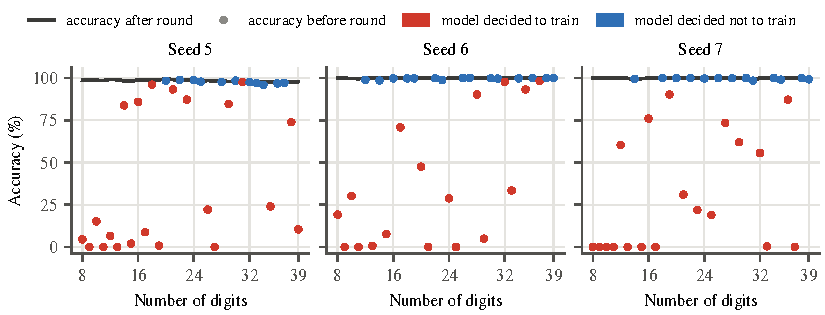
\includegraphics[width=\linewidth]{generated/figure_ladder_decisions.pdf}
\caption{The self-paced arm's decisions. Each circle is one length: the
  accuracy of the model's direct answers just before the round that would
  teach it, red where the model then trained and blue where it did not. The
  line is the accuracy after that round.}
\label{fig:ladder-decisions}
\end{figure}


In the fourth arm the model decides before each round, without correct
answers, where it still has something to learn.
Figure~\ref{fig:ladder-decisions} sets each decision beside the model's
actual accuracy, which it never sees: where it decided not to train, it
already stood where it would end up; where it decided to train, there was a
gap, and training closed it. The arm
learned all four stages on all three seeds while skipping
\gpLadSkippedSeedFive, \gpLadSkippedSeedSix, and \gpLadSkippedSeedSeven{} of
the 32 lengths. It used \gpLadUpdatesShareSeedFive,
\gpLadUpdatesShareSeedSix, and \gpLadUpdatesShareSeedSeven\% of the third
arm's training updates and \gpLadGpuShareSeedFive, \gpLadGpuShareSeedSix,
and \gpLadGpuShareSeedSeven\% of its GPU time, and its final accuracy over 8
to 39 digits differed from the third arm's by $\gpLadDiffMeanSeedFive$,
$\gpLadDiffMeanSeedSix$, and $\gpLadDiffMeanSeedSeven$ points
(Appendix~\ref{app:ladder}, Table~\ref{tab:ladder-pace}). At every skipped length it already answered at
least \gpLadSkippedDirectLowest\% of sums directly, and none fell below
\gpLadSkippedLaterLowest\% in any later round; at the \gpLadWouldSkip{}
lengths where the rule would have skipped in the third arm, building raised
accuracy by only $\gpLadWouldSkipGainMean$ points on average. As in
Section~\ref{sec:novelty-bound}, novelty worked as a quantity: over the
\gpLadNoveltyGapCases{} lengths of the third arm it differed from the gain
the round then produced by \gpLadNoveltyGapMedian{} points at the median and
\gpLadNoveltyGapHigh{} at most.
